%==============================================================================
\section{Formula\c{c}\~{a}o do Problema}
\label{sec:formulacao_problema}
%==============================================================================
Numa solução de integração, baseada no estilo arquitetural \emph{Pipes\&Filters}~\cite{alexander1977}, os \textit{pipes} são representados por canais de mensagens e os \textit{filters} por tarefas atômicas que implementam um padrão de integração concreto e processam dados encapsulados em mensagens.
% A Figura~\ref{fig:pipes-filters} representa esse estilo arquitetural.
%\begin{figure}[htb]
%	\centering
%	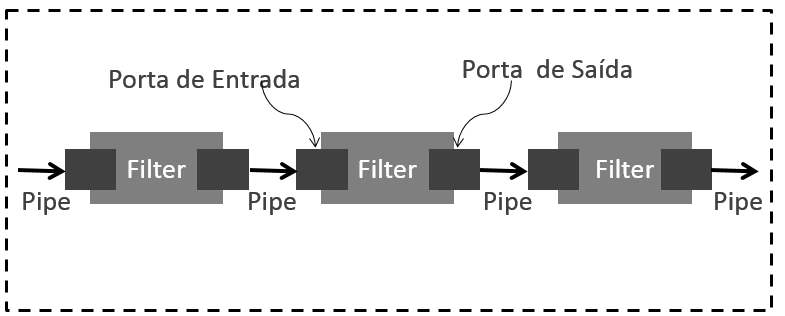
\includegraphics[width=\linewidth]{./figs/pipes_filters.png}
%	\caption{Estilo arquitetural \emph{Pipes\&Filters}}
%	\label{fig:pipes-filters}
%\end{figure}
A Figura~\ref{fig:sample-cafe} mostra o modelo conceitual de uma solução de integração para o problema Café, introduzido por Gregor Hohpe~\cite{hohpe2005} modelado com Guaraná~\cite{frantz2016}.
\begin{figure}[htb]
	\centering
	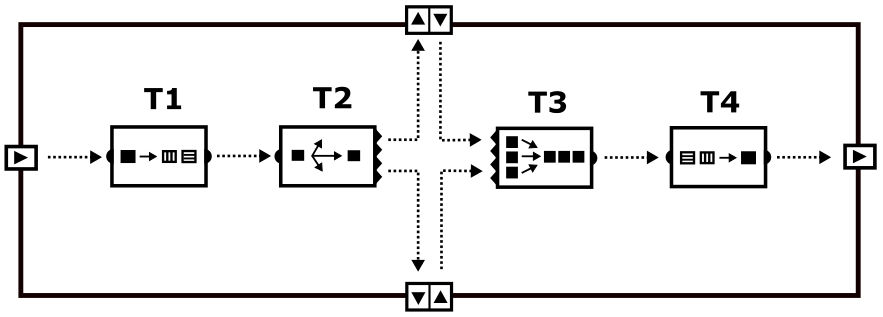
\includegraphics[scale=0.25]{./figs/cafe-guarana.png}
	%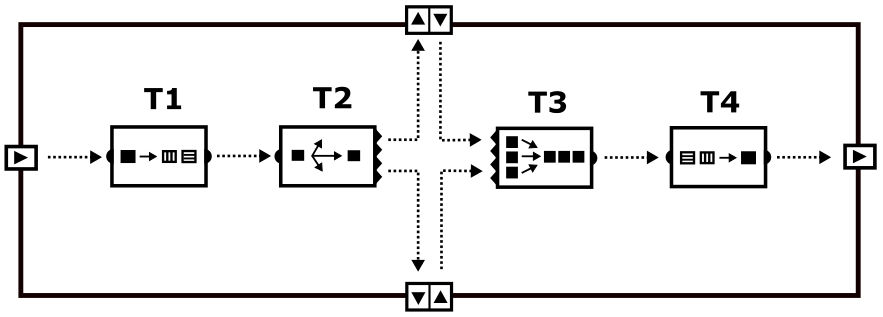
\includegraphics[width=\linewidth]{./figs/cafe-guarana.png}
	\caption{Solução de integração Café}
	%Fonte: \cite{fisher2012spring}
	\label{fig:sample-cafe}
\end{figure}
O modelo conceitual pode ser representado como fluxos de trabalho modelados como Grafos Direcionados Acíclicos, definidos por W(T,E), onde $T = \{t_1,t_2,..t_n\}$ é o conjunto de tarefas e $E$ é o conjunto de arestas direcionadas. Uma aresta $e_{ij}$ da forma $({t_i},{t_j})$ existe, se houver uma dependência de dados entre $t_i$ e $t_j$, onde $t_i$ é tarefa pai de $t_j$ e $t_j$ é tarefa filha de $t_i$. Logo, uma tarefa filha não pode ser executada até que todas as suas tarefas pai estejam concluídas. 
%A Figura~\ref{fig:workflow} mostra fluxos de trabalho da solução de integração Café, onde cada vértice representa uma tarefa e cada aresta possui um peso, que representa o tempo de espera da mensagem na fila de tarefas prontas.
%\begin{figure}[htb]
%	\centering
%	./figs/matrizes-h.pngF
%	%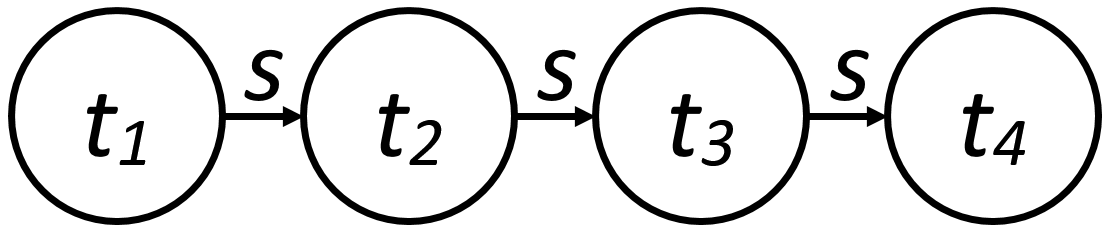
\includegraphics[width=\linewidth]{./figs/workflow.png}
%	\caption{Workflow da solução de integração Café.}
%	\label{fig:workflow}
%\end{figure}
Considera-se que o motor de execução oferece uma variedade de recursos computacionais para execução das tarefas da solução de integração. Essa variedade de recursos é definida por \emph{pool} de \emph{threads}, com diferentes números de \emph{threads}, onde uma \emph{thread} é a unidade básica de processamento. Assim, assume-se que um motor de execução pode ter mais de um \emph{pool} de \emph{threads} e que o número de \emph{threads} em cada um pode ser diferente, ou seja, um \emph{pool} com uma quantidade \textit{x} \emph{threads} e outro com uma quantidade \textit{y}. Considera-se ainda, que um motor de execução tem uma quantidade limitada de recursos computacionais ${\delta _r}$, sendo um recurso computacional $Pool$, um \emph{pool} de \emph{threads} que tem um tipo $Pool _i$, uma capacidade de processamento $PPool_j$. O tipo diferencia os \emph{pools}, a capacidade de processamento é a quantidade de \emph{threads} do \emph{pool}. A capacidade de memória não é tratada; assume-se que é suficiente para executar as tarefas do fluxo de trabalho. Assume-se que para cada tipo de recurso, a capacidade de processamento é definida em termos de instruções por ciclo (IPC), que pode ser estimada~\cite{abraham2016runtime}. Esta informação é usada no algoritmo, para calcular o tempo de execução de uma tarefa em um determinado \emph{pool} de \emph{threads} $Pool$. A variação do desempenho pode ser modelada pelo ajuste da capacidade do $Pool$ e introduzindo uma degradação de desempenho $deg_{Pool_{j}}$ ~\cite{rodriguez2014}. 
O tempo de execução $TE_{{t_i}}^{Poo{l_j}}$ da tarefa $t_i$ em um $Pool$ de tipo $Pool_j$ é estimado pelo tamanho $Ta{m_{{t_i}}}$ da tarefa em instruções por ciclo (IPC), calculado pela Equação~\ref{equa:tempo-execucao}. 
\begin{equation}
TE_{{t_i}}^{Pool_{j}} = Ta{m_{{t_i}}}/({P_{Pool_{j}}}*(1 - {\deg _{Pool_{j}}}))
\label{equa:tempo-execucao}
\end{equation}
%onde:
%
%$Ta{m_{{t_i}}}$ = tamanho da tarefa
%
%$ {P_{Poo{l_j}}} $ = capacidade de processamento do \emph{pool} de threads
%
%$ {\deg _{Poo{l_j}}} $ = degradação de desempenho
O tempo médio de espera na fila de tarefas $TF{i_{e_{ij}}}$ é definido como o tempo para transferir dados entre uma tarefa pai $t_i$ e sua tarefa filha $t_j$ e assume-se que ele pode ser monitorado e medido.  

Finalmente, o tempo total de processamento $TP_{{t_i}}^{Poo{l_j}}$ de uma tarefa em um $Pool$ é calculado na Equação~\ref{equa:tempo-processamento}, onde k é o número de arestas, $t_i$ é uma tarefa pai e $s_k$ representa o tempo gasto pelo motor na troca de \emph{pool} de threads, de maneira que $s_k$ = 0, quando $t_i$ e $t_j$ são processadas no mesmo \emph{pool} e  $s_k$ = 1, caso contrário.
\begin{equation}
TP_{{t_i}}^{Poo{l_j}} = TE_{{t_i}}^{Poo{l_j}} + (\sum\limits_1^k {T{F_{ij}} + {s_k}} )
\label{equa:tempo-processamento}
\end{equation}
%onde:
%
%$ TE_{{t_i}}^{Poo{l_j}} $ = tempo de execução da tarefa em um determinado \emph{pool} de threads.
%
%$TF{i_{e_ij}}$  = tempo de espera na fila de tarefas, ou seja, tempo que para transferir dados entre uma tarefa e sua tarefa filha. 
%
%$ {s_k} $ = tempo gasto na troca de \emph{pool} de threads.
%
%$ k $ =  número de arestas em que uma tarefa é uma tarefa pai. 
O objetivo é encontrar um agendamento de tarefas que possibilite executar as tarefas da solução de integração em \emph{pools} de \emph{threads} do motor de execução, minimizando o tempo total de execução e sem aumentar a quantidade de recursos computacionais. O agendamento de tarefas é definido por $A= (R, M, TR, TTE)$, sendo $R$ um conjunto de recursos; $M$ o mapeamento de tarefas em recursos, $TR$, $TR=\arrowvert R\arrowvert =n$, o total de recursos, $TTE$ o tempo total de execução. Um exemplo é mostrado na Figura~\ref{fig:grafico-mapeamento}, representando o agendamento para o fluxo de trabalho, em que cada uma das quatro tarefas é mapeada para ser executada por um dos três recursos disponíveis, e onde as tarefas pais são executadas antes das sua tarefas filhas, mantendo assim a dependência dos dados.
\begin{figure}[htb]
	\centering
	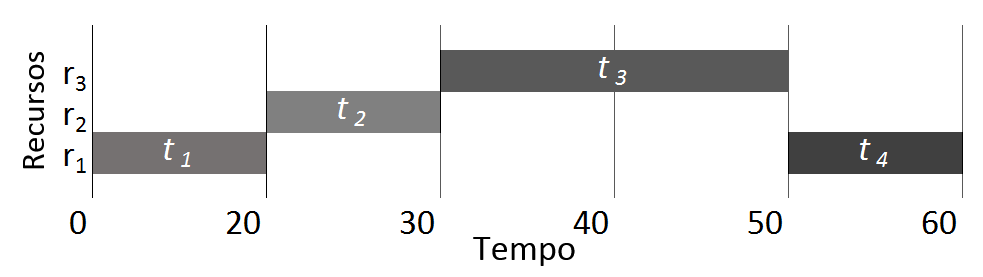
\includegraphics[scale=0.2]{./figs/grafico-mapeamento.png}
	%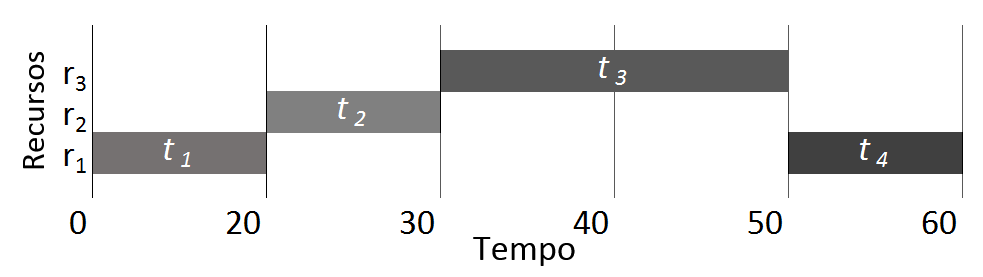
\includegraphics[width=\linewidth]{./figs/grafico-mapeamento.png}
	\caption{Agendamento para o workflow do Café.}
	\label{fig:grafico-mapeamento}
\end{figure}
$R = \{ {r_1},{r_2},...,{r_n}\}$  é o conjunto de recursos (\emph{pools} de \emph{threads}) do motor de execução, onde cada recurso $r_i$ tem associado a ele um $Pool$ do tipo $Pool_i$, um tempo de início estimado para alocação do recurso estimado ${TIni_{r_i}}$. e um tempo de finalização estimado ${TFim_{r_i}}$. M representa um mapeamento para cada uma das tarefas do fluxo de trabalho e é constituído por tuplas $ m_{{t_i}}^{{r_j}} = ({t_i},{r_j},TIn{i_{{t_i}}},TFi{n_{{t_i}}})$, significando que a tarefa $t_i$ será executada pelo recurso $r_j$, com o início da execução agendado para $ TIn{i_{{t_i}}} $ e previsão de término em $ TFi{n_{{t_i}}} $. A Equação~\ref{equa:tempo-total-execução} mostra como o tempo total de execução $ TTE $ é calculado:
\begin{equation}
TTE = \max \{ TFi{m_{{t_i}}}:{t_i} \in T\} 
\label{equa:tempo-total-execução}
\end{equation}
Assim, o problema pode ser formulado como: \textit{encontrar um agendamento $A$ com o menor tempo total de execução $TTE$ da solução de integração, sem exceder um valor pré-definido para o total de recursos $TR$}. Essa formulação é representada pela Equação~\ref{equa:problema}:
\begin{equation}
Minimize {TTE} 
\label{equa:problema}
\end{equation}
\begin{center}
	 sujeito a ${TR \le {\delta _r}} $
\end{center}
